\documentclass{pracamgr}
\usepackage{fontspec}
\usepackage[protrusion=true]{microtype} % does not work with xetex older than 0.9997
\usepackage{polski}
\usepackage{algorithm2e}
\usepackage{amsfonts}
\usepackage{enumitem}
\usepackage{url}
%\usepackage[debugshow]{graphicx}

%\setmainfont[Mapping=tex-text]{DejaVu Serif}
\newfontface\cyr{Hirmos Ponomar}
\newfontface\lat{DejaVu Serif}

% TODO przed wysłaniem:
% - search TODO
% - makro dodaj spacje
% - ' i ' → ' i~', tak samo dla z w o a u
% cerkiewno\-{}słowiański
% - → --

%%% tak się robi listy bez odstępów
%\begin{enumerate}[noitemsep,topsep=0pt,parsep=0pt,partopsep=0pt]
%\end{enumerate}

\newcommand{\quoted}[1]{{\textnormal{\texttt{"#1"}}}}

\renewcommand{\chaptername}{Rozdział} % fix for ugly 'ł'

\author{Mikołaj Dądela}
\nralbumu{262484}

%\setlength{\emergencystretch}{0em}
\pretolerance=1000
\tolerance=10000

\title{Corthus -- korpus równoległy z~interfejsem internetowym
  i~przeszukiwarką fonetyczną}
\tytulang{Corthus -- a~parallel corpus with internet interface and
  a~phonetic search engine}

\kierunek{Informatyka}
\opiekun{dra hab. Adama Przepiórkowskiego\\ Instytut Informatyki}
\date{Wrzesień 2012}

\dziedzina{11.3 Informatyka} % wg klasyfikacji Socrates-Erasmus
\klasyfikacja{ H. Information Systems \\
               H.3 Information Storage and Retreival \\
               H.3.1 Content Analysis and Indexing } % wg ACM

\keywords{tłumaczenie, korpus, dopasowanie, alignment, teksty
  równoległe, wyszukiwanie fonetyczne, metaphone, Python}

\begin{document}
\maketitle

\begin{abstract}
  Praca opisuje tworzenie korpusu równoległego z~tekstów liturgicznych
  w~językach polskim, cerkiewno\-{}słowiańskim
  i~staro\-{}greckim. Korpus został wyposażony w~dwa interfejsy:
  wiersza poleceń oraz internetowy. Zostało zaimplementowane
  przeszukiwanie oparte na przybliżonej wymowie słów, aby można
  było było łatwo znaleźć słowo, którego zna się tylko wymowę.
\end{abstract}

\tableofcontents
%\listoffigures
%\listoftables

%%%%%%%%%%%%%%%%%%%%%%%%%%%%%%%%%%%%%%%%%%%%%%%%%%%%%%%%%%%%%%%%%%%%%%

\chapter*{Wprowadzenie}
\addcontentsline{toc}{chapter}{Wprowadzenie}

\section*{Cel}\label{cel}
\addcontentsline{toc}{section}{Cel}

Głównym celem mojego projektu było ułatwienie szerszej publiczności
dostępu do tekstów liturgicznych w~różnych językach i~sprawienie, żeby
były zrozumiałe dzięki możliwości równoległego ich czytania i~łatwo
dostępne dzięki wyszukiwarce.

Pragnąłem również ułatwić zainteresowanym naukę języka
cerkiewno\-{}słowiańskiego, poczynając już od pierwszego jej etapu,
którym jest nauka czytania. Chciałem również poprzez zestawienie
tekstów unaocznić analogiczny, a często identyczny szyk zdań
w~językach starogreckim i~cerkiewno\-{}słowiańskim. Trwa obecnie
dyskusja na temat zasadności tłumaczenia tekstów liturgicznych na
język polski i~poprawności istniejących tłumaczeń -- chciałem więc
stworzyć pomoc do ich badania, jak również do potencjalnego
tłumaczenia kolejnych podobnych tekstów na język polski.

Dużym wyzwaniem w~realizacji projektu okazało się dopasowywanie
tekstów wielojęzycznych, gdyż teksty liturgiczne w~zależności od ich
redakcji bardzo się różnią. Chciałbym więc również przedstawić
algorytmy dopasowywania tekstów użyte w~niniejszej pracy. Poświęcam
temu zagadnieniu osobny rozdział.

\section*{Wizja}
\addcontentsline{toc}{section}{Wizja}

Planowałem stworzyć serwis internetowy, w~którym można łatwo
przeglądać, przeszukiwać i~porównywać teksty w~różnych językach,
w~pisowni oryginalnej lub w~transkrypcji fonetycznej na język polski.

Ważnym elementem projektowanego serwisu była przeszukiwarka
wspomnianych tekstów. Głównym jej celem była nie tyle precyzja
wyszukiwania, co łatwość jej użycia, gdyż pisownia cerkiewno\-{}słowiańska
i~starogrecka jest na tyle skomplikowana, że nie można założyć, że
użytkownik bezbłędnie wpisze w~wyszukiwarkę frazę z~szukanego tekstu.

Ciekawą możliwością dalszego rozwinięcia projektu byłaby implementacja
rytmu kalendarza prawosławnego i~udostępnienie linku „tekst na
dzisiaj".

Mimo że teksty liturgiczne są głównym przedmiotem zainteresowania
niniejszej pracy, to starałem się stworzyć na tyle ogólną
implementację, żeby można było jej później użyć do innych zastosowań,
np. stworzenia bazy tłumaczeń tekstów technicznych. Niektóre algorytmy
(na przykład podział na zdania, transliteracja) w~sposób nieunikniony
występują w różnych wersjach dla trzech różnych języków, z~których
składał się korpus, ale nic nie stoi na przeszkodzie, żeby dodać
analogiczne funkcje do obsługi następnych języków.


\section*{Zarys pracy}
\addcontentsline{toc}{section}{Zarys pracy}

W pracy zostało zaimplementowane automatyczne dopasowywanie tekstów, z
możliwością łatwego ręcznego wprowadzania poprawek. Algorytmy używane
do dopasowywania tekstów zostały opisane w rozdziale \ref{r:algo}.

System został wyposażony w interfejs internetowy, w którym użytkownik
może otworzyć wybrany tekst, jak również przeszukiwać bazę tekstów
używając przybliżonej wymowy słów, a nie ich dokładnej
pisowni. Dopasowanie tekstów zostało unaocznione poprzez złożenie
tekstów w jedną tabelę i dynamiczne podświetlanie odpowiadających
sobie elementów tekstu. Została również zaimplementowana transkrypcja
fonetyczna z języków obcych na polski, aby uczynić teksty
przystępniejszymi dla tych użytkowników, którzy nie potrafią szybko
czytać tekstu cerkiewno\-{}słowiańskiego lub greckiego. Wszystkie
wspomniane części projektu zostały szczegółowo opisane w rozdziale
\ref{r:opis}. Dodatek \ref{r:formaty} zawiera dodatkowy opis formatów
plików użytych w projekcie.


\section*{Nota licencyjna}
\addcontentsline{toc}{section}{Nota licencyjna}

Kod źródłowy systemu zostaje udostępniony na warunkach licencji Apache
2.0, której warunki zostały załączone w dodatku \ref{r:licencja}.

%\section*{Definicje} % TODO!
%\addcontentsline{toc}{section}{Definicje}
%
%\paragraph{Tekst} ciąg znaków Unicode.
%
%\paragraph{Dopasowanie dwóch tekstów} Ciąg par $<s_a, s_b>$, gdzie
%$s_a$ i~$s_b$ są zdaniami z~odpowiednich tekstów. $s_a$ lub $s_b$ mogą
%być też puste, jeśli dany fragment został pominięty w~jednym z~tekstów.



%%%%%%%%%%%%%%%%%%%%%%%%%%%%%%%%%%%%%%%%%%%%%%%%%%%%%%%%%%%%%%%%%%%%%%

\chapter{Algorytmy dopasowania tekstów}\label{r:algo}

Aby zbiór tekstów w~różnych językach można było nazwać korpusem
równoległym, teksty muszą być do siebie
dopasowane. Dopasowanie\footnote{czasem też nazywane wyrównaniem,
  z ang. \textit{alignment}} tekstów równoległych polega na określaniu
odpowiadających sobie zdań w~poszczególnych językach. Jest to
potrzebne do prowadzenia badań lingwistycznych.

Dopasowanie tekstów nie jest jednak zadaniem trywialnym, gdyż podczas
tłumaczenia dwa zdania mogą być sklejone w~jedno lub jedno może być
podzielone na dwa; zdarzają się też opuszczenia i~wstawienia nowych
zdań. Jest to szczególnie trudne w~tekstach liturgicznych, gdyż,
w~zależności od redakcji, często powtarzające się fragmenty mogą być
podane w~całości lub skrócone do kilku pierwszych słów; na przykład
refren może być podany raz lub też powtórzony po każdej zwrotce
pieśni. Zdarzają się też duże fragmenty didaskaliów, które występują
tylko w~jednej wersji językowej.

Program dopasowujący teksty w~niniejszej pracy opiera się na
algorytmie korzystającym z~funkcji $D$ szacującej prawdopodobieństwo
dopasowania zdań (nazywanej też funkcją podobieństwa), bazując na
pamięci tłumaczeniowej $TM$.

\section{Algorytm dynamiczny}

Jednym z~algorytmów, które pozwalają na wygenerowanie dopasowania
tekstów, jest algorytm dopasowywania sekwencji opierający się na
technice programowania dynamicznego. Jedną z~jego wersji, dostosowaną
właśnie do dopasowywania zdań można znaleźć w~pracy
\cite{church+gale}. Algorytm ten i~jemu podobne są używane w~wielu
różnych zastosowaniach, na przykład w~bioinformatyce do zestawiania
sekwencji genetycznych czy w~odnajdywaniu podobnych wzorców
w~sekwencjach audio i~wideo (znany jako Dynamic time warping).

Algorytm ten bazuje na funkcji kosztu, która ocenia podobieństwo dwóch
dopasowywanych zdań (duże podobieństwo -- niski koszt
przyporządkowania). Algorytm w~jego najprostszej wersji można zapisać
w~ten sposób:

\begin{algorithm}[H]

  \KwIn{$A = a_1, \ldots, a_n$}
  \KwIn{$B = b_1, \ldots, b_m$}

  $cost \leftarrow \mbox{macierz zerowa}\ n \times m$ \;
  $cost_{0, 0} \leftarrow 0$ \;
  \ForEach{$i \in 1\ ..\ n\mathrm{-}1$}{
    \ForEach{$j \in 1\ ..\ m\mathrm{-}1$}{
      $c \leftarrow \infty$ \;
      \If{$i > 0 \wedge j > 0$}{
        $c \leftarrow \min(c, \:cost_{i-1, j-1} - \log D(a_{i-1}, b_{j-1}))$ \tcp*{dopasowanie $a_{i-1}$ do $b_{j-1}$}
      }
      \If{$i > 0$}{
        $c \leftarrow \min(c, \:cost_{i-1, j} - \log D(a_{i-1}, null))$ \tcp*{opuszczenie $a_{i-1}$}
      }
      \If{$j > 0$}{
        $c \leftarrow \min(c, \:cost_{i, j-1} - \log D(null, b_{j-1}))$ \tcp*{opuszczenie $b_{j-1}$}
      }
      $cost_{i, j} \leftarrow c$
   }
 }
 \KwRet{$cost_{m-1, n-1}$} \;

\end{algorithm}

Podana wersja zwraca tylko całkowity koszt dopasowania. Jest to
uproszczenie algorytmu, ponieważ przy dopasowywaniu tekstów, zależy
nam przede wszystkim na przyporządkowaniu zdań, a całkowity koszt tego
przyporządkowania jest mniej istotny. Pominięte zostały również inne
rodzaje ,,skoków'', potrzebne dla przyporządkowań 2 do 2 lub 1 do 3
zdań. Pomijam jednak te szczegóły na rzecz czytelności kodu -- zasada
działania algorytmu pozostaje ta sama.

Używaną funkcją kosztu jest funkcja $-\log p_k$, gdzie $p_k =
D(a_i, b_j)$ jest prawdopodobieństwem, że zdanie $a_i$
jest tłumaczeniem $b_j$, ozn. $a_i \sim b_j$. Zsumowany
koszt dopasowania całego tekstu jest więc logarytmem iloczynu
wspomnianych prawdopodobieństw, czyli estymowanego prawdopodobieństwa
poprawnego dopasowania całego tekstu.

\section{Funkcja podobieństwa $D$}

Kluczowa dla skutecznego działania powyższego algorytmu jest
oczywiście dobrze dobrana funkcja podobieństwa $D(a_i, b_j)$.

Funkcja podobieństwa $D$ zastosowana w~niniejszej pracy opiera się
głównie na parach tłumaczeń. Korzysta ona z~pamięci tłumaczeniowej
$TM : L \times L \mapsto [0, 1]$. Jest to zbiór par $(a_i, b_j)$
z~przyporządkowanymi prawdopodobieństwami
$\mathbb{P} (a_i \sim b_j | a_i, b_j)$, gdzie
$a_i \sim b_j$ oznacza ,,$a_i$ jest tłumaczeniem $b_j$’’.

$TM$ jest funkcją zdefiniowaną dla wszystkich par napisów, i~dla
nieznanych par zwraca zawsze małe, niezerowe prawdopodobieństwo. Aby
jednak rozróżnić napisy bardziej i~mniej prawdopodobne, w~przypadku
nieznalezienia pary zdań w~pamięci $TM$ funkcja $D$ mnoży zwrócone
prawdopodobieństwo o~własną, heurystyczną ocenę podobieństwa zdań.

Ocena ta opiera się na założeniu (nieprawdziwym), że zawsze jedno
słowo w~pierwszym zdaniu odpowiada jednemu słowu w~drugim
zdaniu. Jeśli nie da się słów w~ten sposób dopasować, bo zdania różnią
się długością, to przyjmujemy, że słowa z~któregoś zdania zostały
usunięte. Prawdopodobieństwo takiego dopasowania wynosi więc
$p_m{}^{\min(k, l)} * p_r{}^{|k-l|}$, gdzie $p_m$ jest prawdopodobieństwem
dopasowania dwóch słów, a $p_r$ jest prawdopodobieństwem usunięcia
słowa. W~swojej pracy przyjąłem arbitralnie, że $p_m = 0.5, p_r =
0.2$.

Taka ocena odpowiada spostrzeżeniom z~pracy \cite{church+gale}, że
długości odpowiadających sobie zdań są bardzo silnie skorelowane.

\section{Pamięć tłumaczeniowa $TM$}

Pamięć tłumaczeniowa $TM$ przechowuje często występujące pary
tłumaczeń zdań, wraz z~ich częstościami występowania i~prawdopodobieństwami,
że zdania w~parze są rzeczywiście swoimi tłumaczeniami.

Aby jednak można było znaleźć często występujące pary tłumaczeń,
potrzebne jest dopasowanie tekstów -- koło się zamyka. Na szczęście
wśród tekstów w~bazie są takie, które można dopasować, bazując tylko
na ich długościach. Teksty te zostały więc dopasowane za pomocą
Hunaligna\footnote{Więcej o tym narzędziu można przeczytać w~punkcie
  \ref{r:hunalign} i w internecie na stronie \cite{hunalign}.},
i~początkowa pamięć tłumaczeniowa bazowała właśnie na tym pierwszym
dopasowaniu. Zapisywane były tylko pary, które wystąpiły co najmniej 2
razy. Tak dopasowane zdania stanowią dla przeciętnego tekstu polskiego
4,20\% całości, 4,18\% dla cerkiewno\-{}słowiańskiego i~4,84\% dla
greckiego.

Kiedy wspomniane pary tłumaczeń są już gotowe, prawdopodobieństwa
można obliczyć w~następujący sposób:
$$
\mathbb{P}( a_i \sim b_j | a_i, b_j)
=
\frac{ \mathbb{P}( a_i \sim b_j, a_i, b_j)}
     { \mathbb{P}( a_i, b_j) }
=
\frac{ \mathbb{P}( a_i \sim b_j ) }
     { \mathbb{P}(a_i) +  \mathbb{P}(b_j) }
=
\frac{ \#( (a_i, b_j) ) }
     { \#(a_i) + \#(b_j) } ,
$$
gdzie $\#$ oznacza liczbę wystąpień w~korpusie odpowiednio zdania lub
pary zdań, a zapis $a_i \sim b_j$ oznacza zdarzenie ,,zdanie $a_i$ jest
tłumaczeniem zdania $b_j$''.

Tak obliczone prawdopodobieństwo jest bardzo sensownym wnioskiem,
jednak okazuje się ono niepraktyczne, gdyż pamięć tłumaczeniowa
zapytana o~parę, w~której będzie znała tylko jedno ze zdań, zwróci
zerowe prawdopodobieństwo, które spowoduje nieskończony koszt
dopasowania. Co gorsza, jeśli oba zdania będą nieznane, podjęta będzie
niebezpieczna próba dzielenia przez zero. Aby rozwiązać oba powyższe
problemy, stosuje się
tzw. wygładzanie\footnote{ang. \textit{smoothing}}. W~niniejszej pracy
zastosowane zostało wygładzanie Laplace’a -- wzór przyjmuje wtedy
postać:
$$
\mathbb{P}( a_i \sim b_j | a_i, b_j)
=
\frac{ \#( (a_i, b_j) ) + \alpha }
     { \#(a_i) + \#(b_j) + \alpha N } ,
$$
gdzie $N$ to liczba możliwych par utworzonych z~dopasowanych zdań, a
$\alpha$ jest małą liczbą dodatnią.

Po utworzeniu pamięci tłumaczeniowej okazało się, że w~bazie znajduje
się wiele różnych pisowni tego samego akapitu (patrz
Rys. \ref{fig:pisownia}) -- aby więc temu zaradzić, wszystkie akapity
są przed przetwarzaniem zamienione na ciągi kluczy
Metaphone\footnote{Dokładny opis tego algorytmu można znaleźć w~punkcie
  \ref{r:metaphone}.}.

\begin{figure}[h]
  \small
  \caption{Różne wersje pisowni tego samego akapitu}
  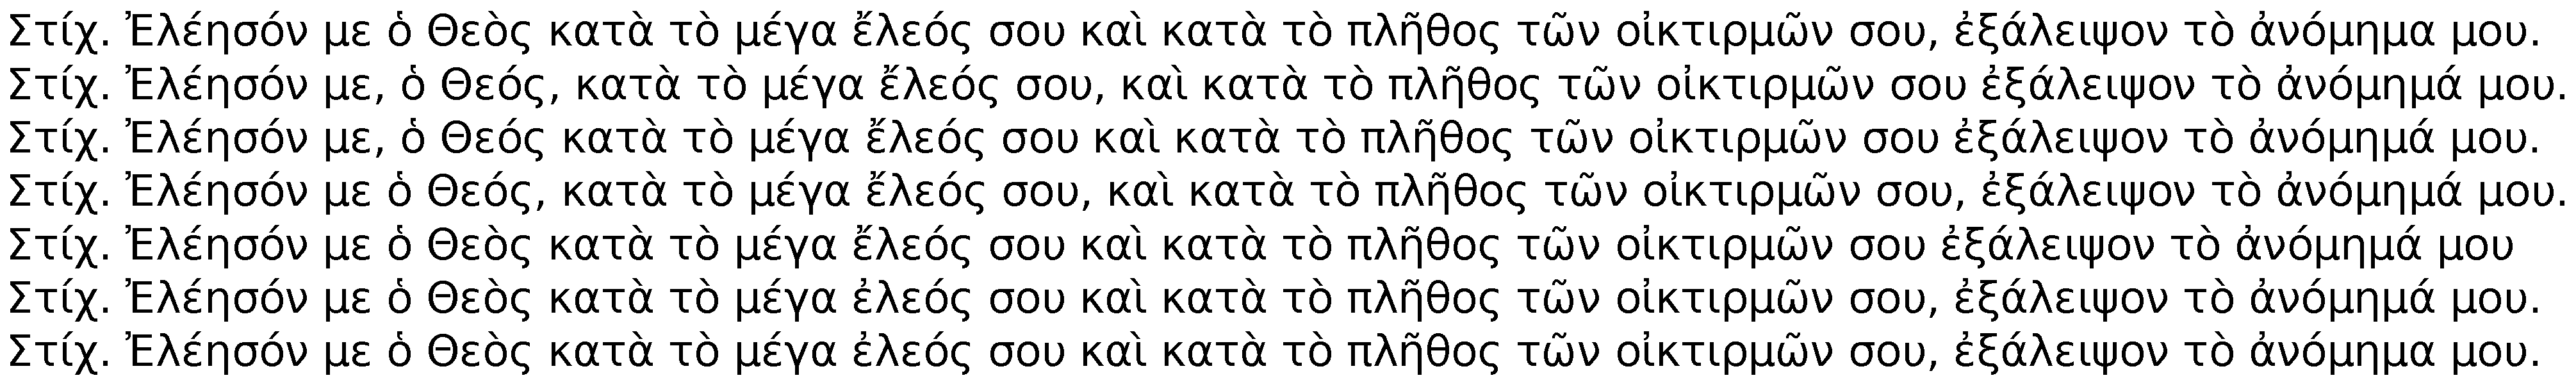
\includegraphics[width=\textwidth]{pisownia.eps}
  \label{fig:pisownia}
\end{figure}

\section{Poprawianie dopasowań}

Aby poprawić błędy w automatycznie wygenerowanym dopasowaniu, została
opracowana następująca metoda: najpierw człowiek wskazuje zbiór par
zdań, które powinny się znaleźć w dopasowaniu, a następnie algorytm
dopasowuje fragmenty pomiędzy nimi. Poza -- oczywiście -- lepszym
dopasowaniem, skraca to też w znaczący sposób czas działania programu
dopasowującego, z powodu złożoności jego algorytmu $\mathcal{O}(n^2)$.



%Na początku potrzebne było dopasowanie tekstów na poziomie plików. Nie
%było to trywialne, bo teksty były różnie zredagowane, i~bardzo często
%jeden plik odpowiadał kilku plikom w~innym języku. Wykonałem to
%zadanie ręcznie, z~pomocą prostego skryptu dzielącego plik na części w
%odpowiednich miejscach.

\section{Dopasowanie wstępne}

Jak łatwo zauważyć, powyższy algorytm ma złożoność obliczeniową
$\mathcal{O}(n^2)$. Aby poprawić jego wydajność, zaimplementowane
zostało wstępne dopasowywanie tekstów. Zasada jego działania jest
prosta: w~obu tekstach wyszukiwane są fragmenty, które występują
w~parach $TM$, a następnie dopasowane są sekwencje tych
fragmentów. Dzięki temu zamiast dopasowywać od razu cały tekst, można
dopasowywać za jednym razem tylko jego małe fragmenty, co znacznie
obniża oczekiwany czas działania programu (mimo że pesymistyczny jest
wciąż taki sam) -- analogicznie jak przy ręcznym poprawianiu dopasowań
przedstawionym powyżej. Często to wstępne dopasowanie prowadzi również do
poprawienia poprawności dopasowania. Bardzo dobitnie ukazuje to
zjawisko rysunek \ref{fig:matrix}.

\begin{figure}[p]
  \small
  \caption{Macierz kosztów}
  \includegraphics[width=\textwidth]{koszty.png}

  \setlength\parindent{20pt}

  Macierz kosztów dla dopasowania poszczególnych zdań tekstu {\tt
  kanon\_izr}, w~językach polskim i~cerkiewno-słowiańskim. Oś X
  odpowiada zdaniom tekstu polskiego, oś Y -- zdaniom tekstu
  cerkiewno-słowiańskiego. Kolor piksela $(i, j)$ obrazka odzwierciedla
  koszt dopasowania zdania $a_i$ do $b_j$ (nie jest to więc zsumowany
  koszt, przechowywany w~tablicy $cost$ algorytmu).

  Dwa przedstawione wykresy ukazują dwa tryby działania algorytmu --
  po lewej widoczna jest pełna macierz kosztów, którą oblicza algorytm
  w~podstawowej wersji. Po prawej ukazany jest wynik działania
  programu, w~wersji ze wstępnym dopasowaniem dobrze pasujących fraz,
  i~odpowiednie fragmenty macierzy kosztów, które są wtedy obliczane.

  Ścieżka złożona z~kółek biegnąca przez wykres oznacza wygenerowane
  dopasowanie tekstów -- każdy jej punkt to przyporządkowanie sobie
  zdań. Ścieżka złożona z~punktów oznacza poprawne, wzorcowe
  dopasowanie. Ścieżki nie są ciągłe w~miejscach, gdzie mamy do
  czynienia z~dopasowaniem wielu zdań (notabene, w~przypadku takich
  dopasowań koszt jest liczony dla połączonych zdań, więc inaczej, niż
  ukazuje wykres).

  Ciemniejsze poziome i~pionowe paski odpowiadają dłuższym zdaniom,
  ponieważ koszt dopasowania zdań jest bardzo silnie skorelowany z~ich
  długością. Pary zdań, które występują w~$TM$ nie wyróżniają się na
  tym wykresie (mają niemal biały kolor, który łatwo się gubi
  w~jasnoszarym otoczeniu).

  Wyniki dla lewego wykresu: precision: 67,30\%, recall: 66,73\%

  Wyniki dla prawego wykresu: precision: 81,71\%, recall: 89,22\%

  \label{fig:matrix}
\end{figure}

\begin{figure}[h]
  \centering \small
  \caption{Pary indeksów dla przedstawionego dopasowania:
    $(0,0),$ $(1,1),$ $(2, 3),$ $(5, 4)$}
  \includegraphics[height=1.3in]{pairs.eps}
  \label{fig:pairs}
\end{figure}

\begin{figure}[h]
  \centering \small
  \caption{Pary zbiorów indeksów dla przedstawionego dopasowania:
    $(\{1\},\{1\}),$ $(\{2\},\{2,3\}),$ $(\{3,4,5\},\{4\})$}
  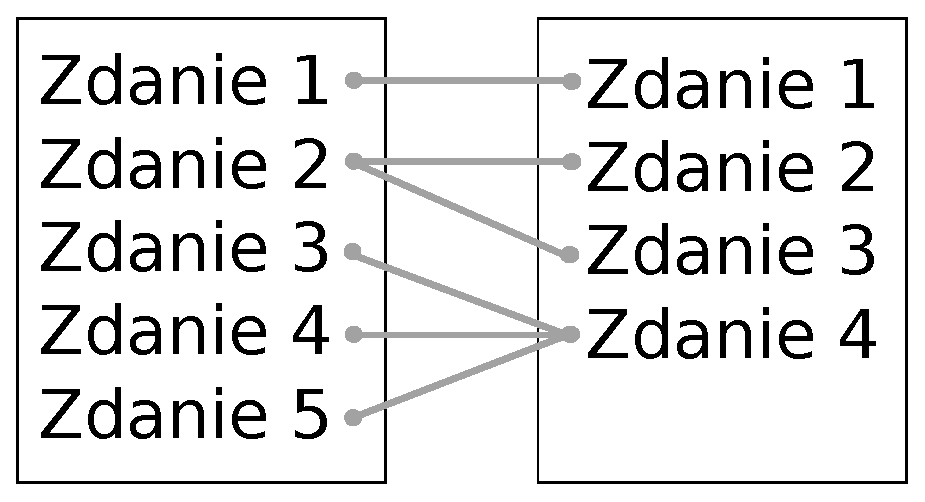
\includegraphics[height=1.3in]{setpairs.eps}
  \label{fig:setpairs}
\end{figure}

\section{Scalanie dopasowań}

Aby wyświetlić jednocześnie teksty w~trzech językach, potrzebowałem
scalić ze sobą dopasowania par tekstów w~jedno dopasowanie wszystkich
trzech tekstów jednocześnie.

Prostym podejściem do tego zagadnienia jest wybranie z~wyrównań tych
par zdań, gdzie wszystkie dopasowania są zgodne. Jeśli dopasowania par
tekstów są poprawne, w~wyniku otrzymamy również poprawne dopasowanie.

Można to zapisać jako algorytm w następujący sposób:

\begin{algorithm}[H]
  \KwIn{$A_1 \mathrm{\ -\ dopasowanie\ tekstów\ 1\ i\ 2\ w\ formie\ par\ indeksów\ (patrz\ rys.\ \ref{fig:pairs})}$}
  \KwIn{$A_2 \mathrm{\ -\ dopasowanie\ tekstów\ 2\ i\ 3\ w\ formie\ par\ indeksów}$}
  \KwIn{$A_3 \mathrm{\ -\ dopasowanie\ tekstów\ 1\ i\ 3\ w\ formie\ par\ indeksów}$}
  $M_2 \leftarrow$ mapa utworzona z $A_2$, interpretowanego jako pary klucz-wartość \;
  $A_r \leftarrow \emptyset$ \;
  \ForEach{$(i, j) \in A_1$}{
    \If{$(i, M_2[j]) \in A_3$}{
      $A_r \leftarrow A_r \cup \{(i, j, M_2[j])\}$ \;
    }
  }
  \KwRet{$A_r$}
\end{algorithm}

W~pracy została zastosowana podobna metoda, jednak dla prostoty
scalane są tylko 2 dopasowania: polskiego z~cerkiewno\-{}słowiańskim
i~cerkiewno\-{}słowiańskiego z~greckim.

\pagebreak

\section{Ewaluacja dopasowań}

Ewaluacja dopasowania staje się łatwa, jeśli zamienimy dopasowanie na
zbiór -- wówczas można ocenić dopasowanie używając miar dokładności
i~pełności\footnote{ang. \textit{precision} i~\textit{recall}},
szeroko stosowanych w~systemach uczenia maszynowego. Aby jednak
równomiernie rozłożyć ,,wagę'' dopasowania na wszystkie fragmenty,
potrzebne będą też wagi przy elementach (czyli parach indeksów) tego
zbioru.

Zamiana dopasowania na zbiór (oznaczony dla porządku $S$) przebiega
następująco:

\begin{algorithm}[H]
  \KwIn{$A - \mathrm{dopasowanie\ tekstów\ w\ formie\ par\ zbiorów\ indeksów\ (patrz\ rys.\ \ref{fig:setpairs})}$}
  $S \leftarrow \emptyset$ \;
  $W \leftarrow \mbox{map} : \mathbb{N} \times \mathbb{N} \mapsto [0, 1]$ \;
  \ForEach{$(I, J) - \mathrm{para\ zbiorów\ indeksów\ z\ dopasowania}\ A$  }{
    \lIf{$I = \emptyset$}{ $I \leftarrow \{ \mbox{null} \} $ } \;
    \lIf{$J = \emptyset$}{ $J \leftarrow \{ \mbox{null} \} $ } \;
    $S \leftarrow S \cup (I \times J)$ \;
    \ForEach{$(i, j)\ \in\ I \times J$}{
      $W[i, j] \leftarrow |I| \cdot |J|$
    }
  }
  \KwRet{$S$}
\end{algorithm}

Następnie, kiedy uzyskaliśmy już zbiory par $S_a$, $S_b$ i~wagi $W_a$,
$W_b$ dla odpowiednio wygenero\-{}wanego i~wzorcowego dopasowania, możemy
obliczyć dokładność i~pełność dopasowania:

$$
\mbox{precision} = \frac{\sum_{(i, j)\:\in\:S_a \cap S_b} W_a[i, j]}{|S_a|},\:\:
\mbox{recall}    = \frac{\sum_{(i, j)\:\in\:S_a \cap S_b} W_b[i, j]}{|S_b|}
$$


%%%%%%%%%%%%%%%%%%%%%%%%%%%%%%%%%%%%%%%%%%%%%%%%%%%%%%%%%%%%%%%%%%%%%%

\chapter{Opis projektu}\label{r:opis}

\section{Konwersja danych wejściowych}

Teksty pobrałem ze stron \cite{orthlib}, \cite{analogion} i
\cite{liturgia}. Pliki z~tych stron były odpowiednio w~formatach
HIP\footnote{HIP -- standard zapisu tekstu
  cerkiewno\-{}słowiańskiego. Więcej szczegółów w~dodatku \ref{encoding}},
HTML i~DOC.

Zdecydowałem wszystkie te pliki przekonwertować do zwykłego tekstu
kodowanego w~UTF-8. Napisałem w~tym celu skrypt w~Pythonie, który
korzystał dodatkowo z~Elinksa i~AbiWorda. Zdecydowałem się na
kodowanie UTF-8, bo dzięki niemu mogłem używać jednego kodowania dla
wszystkich plików, i~uznałem, że to uproszczenie rekompensuje 2 razy
większy rozmiar pliku. Decyzja o~przejściu na zwykły tekst oznaczała
również rezygnację z~formatowania. Połamałem akapity na wiersze nie
dłuższe niż 70 znaków, rozdzielając je pustymi wierszami (tak jak w
TeXu), tak żeby można było je wygodnie przeglądać w~dowolnym edytorze
tekstu lub w~konsoli.


\section{Eksperymenty, próby i błędy}

Zacząłem swoją pracę od poszukiwań gotowych narzędzi, które
odpowiadałoby przynajmniej części założeń opisanych powyżej. Postaram
się tu krótko opisać swoje doświadczenia z~nimi.

\paragraph{Hunalign}\label{r:hunalign}
Hunalign \cite{hunalign} jest narzędziem zestawiającym 2 teksty na poziomie zdań
(zakładając, że są już podzielone na zdania), bazując na ich
długościach i~(opcjonalnie) na słowniku. Jeśli jednak nie dysponujemy
słownikiem, można uruchomić Hunaligna z~opcją {\tt -realign} --
Hunalign wówczas po pierwszym, wstępnym dopasowaniu próbuje wygenerować
przybliżony słownik, a następnie dopasowuje teksty ponownie z~użyciem
tego słownika. Dopasowania generowane przez Hunaligna są niemal w
100\% poprawne, jeśli teksty dokładnie sobie odpowiadają. Niestety
teksty, z~którymi pracowałem, bardzo często różniły się od siebie
dużymi fragmentami, co powodowało przesunięcia w~dopasowaniu.

Mimo to Hunalign okazał się bardzo przydatny, gdyż, bazując głównie na
długości zdań, generuje dopasowanie, które może zostać wykorzystane do
zapełnienia pamięci tłumaczeniowej, która następnie może
posłużyć do polepszenia dopasowania.

\paragraph{GIZA++}
To narzędzie \cite{giza} służy do tworzenia dopasowania na poziomie
słów z~już dopasowanych par zdań. Nie użyłem go w~mojej pracy,
ponieważ przede wszystkim potrzebne było dopasowanie na poziomie
zdań. Dopasowanie na poziomie słów byłoby niewątpliwie ciekawym
i~użytecznym rozszerzeniem tej pracy, jest jednak poza jej zakresem.

\paragraph{Poliqarp}
Jest to wolny (i darmowy) zestaw narzędzi do przeszukiwania dużych
korpusów \cite{poliqarp}. Wspiera obsługę korpusów otagowanych
znacznikami morfosyntaktycznymi i~pozwala na przeszukiwanie korpusu za
pomocą złożonych zapytań. W początkowej fazie projektu była planowana
integracja niniejszego projektu z Poliqarpem, jednak teksty, którymi
się zajmowałem w~swojej pracy, nie były otagowane, więc nie mógłbym
też wykorzystać pełni możliwości Poliqarpa. Poliqarp nie posiada
również obsługi korpusów równoległych.

\paragraph{Wzorce odmiany i~lematyzacja}
Próbowałem uprościć Hunalignowi generowanie przybliżonego słownika
poprzez usunięcie końcówek morfosyntaktycznych ze słów. Nie znalazłem
jednak gotowej biblioteki, wykonującej takie zadanie. Rozważałem
ręczną implementację tej funkcjonalności, ale po przyjrzeniu się
skomplikowanym wzorcom odmiany języka cerkiewno\-{}słowiańskiego
\cite{strach} zrezygnowałem. Początkowo przybliżałem lematyzację
skracaniem słowa do 5 liter, a po implementacji Metaphone zauważyłem,
że Metaphone również łączy pod wspólnym kluczem wiele form fleksyjnych
jednego słowa, więc w~końcowej wersji projektu dopasowuję do siebie
nie oryginalne teksty, lecz ciągi kluczy Metaphone z~nich utworzone.

\paragraph{Słowniki}
Szukałem również słownika cerkiewno\-{}słowiańsko-polskiego, lecz
znalazłem tylko jeden \cite{znosko}, autorstwa O. Aleksego Znosko,
i~nie udało mi się go zdobyć w~wersji cyfrowej -- na mail do wydawcy
otrzymałem odpowiedź, że autor zmarł przed wydaniem tego słownika,
i~plik z~zawartością słownika nigdzie się nie zachował.



\section{Architektura katalogów}

Cała implementacja została napisana w~języku Python.

Główna funkcjonalność została umieszczona w~katalogu
\textbf{toolkit}. Wiele skryptów z~tego folderu można wywołać z~wiersza
poleceń, aby wykonać różne zadania (patrz rozdział \ref{r:cli}).

Interfejs internetowy znajduje się w~katalogu \textbf{www}. Został on
szczegółowo opisany w~rozdziale \ref{r:www}.

Katalog \textbf{texts} zawiera wszystkie teksty w~postaci plików
tekstowych, i~odpowiadające im pliki dopasowań. Moja decyzja
o~używaniu plików tekstowych zamiast bazy danych była powodowana
prostotą operacji na plikach w~konsoli, i~możliwością łatwej zmiany
w~organizacji tekstów. Łatwość zmian była dla mnie bardzo ważna, bo
w~początkowej fazie rozwoju projektu nie było jasne, w~jaki sposób
system będzie korzystał z~tekstów.

Nazwa pliku z~tekstem źródłowym ma postać {\tt
  texts/}\textit{książka}{\tt /}\textit{rozdział}{\tt
  /}\textit{język}{\tt .txt}, gdzie \textit{język} jest jednym
spośród ,,pl'', ,,cu''\footnote{,,cu'' oznacza język
  cerkiewnosłowiański, zgodnie ze standardem ISO 639-1.}  i~,,el''.

W katalogu \textbf{data} znajduje się pamięć tłumaczeniowa, oznaczana
wcześniej też symbolem $TM$.

Katalog \textbf{external} zawiera zewnętrzne biblioteki i~narzędzia,
z~których korzysta projekt. Są to Hunalign \cite{hunalign} i~Whoosh
\cite{whoosh}.



\section{Transformacje tekstu}

Aby poprawnie wyświetlić tekst w~języku cerkiewno\-{}słowiańskim,
potrzebna była specjalna czcionka, która oprócz liter zawierała
również zestaw ligatur potrzebnych do poprawnego ułożenia znaków
diakrytycznych nad konkretnymi literami. Przygotowanie tekstu do
wyświetlenia w~takiej czcionce również wymagało napisania prostego
skryptu.

Język cerkiewno\-{}słowiański w~zapisie często występujących słów korzysta
ze skrótów. Polegają one zazwyczaj na opuszczeniu samogłosek
(zazwyczaj tytło proste, {\cyr\ ҃}) lub środkowej części wyrazu
(zazwyczaj tytła literowe, {\cyr ⷭ\ \ ⷢ\ \ ⷣ}). Język
cerkiewno\-{}słowiański korzysta ponadto z~własnego systemu zapisu
liczb. Wobec tego, aby dokonać transkrypcji fonetycznej takiego
tekstu, należało najpierw rozwinąć wszystkie skróty i~zamienić liczby
na cyfry arabskie. Napisałem w~tym celu moduł {\tt translit.expand\_cu},
zawierający listę 130 różnych skrótów i~obsługujący liczby do 10
tysięcy (większe liczby nie występują w~tekstach). Aby konwersja mogła
działać wydajnie, skompilowałem wszystkie wzorce skrótów do jednego
wyrażenia regularnego.

Następnie zaimplementowałem transkrypcję fonetyczną na polski w~module
{\tt cu2pl}. Największy problem sprawiło mi tutaj dostosowanie wyniku
do polskiej pisowni (przede wszystkim chodziło tu o~litery ,,i''
i~,,j'' w różnych kontekstach).

Zaimplementowałem również transkrypcję fonetyczną z~języka
starogreckiego na polski. Dokonuję tej transkrypcji jednak zgodnie
z~regułami wymowy współczesnej greki, dlatego, że w~ten sposób są zwykle
czytane. Konwersja zachodzi w~dwóch etapach: najpierw upraszczam
zapis, usuwając znaki przydechu (dasia, prosgegrammeni, ypogegrammeni)
i~zamieniając wszystkie rodzaje akcentu (tonos, oxia, varia,
perispomeni) na jeden (tonos), i~dopiero wtedy dokonuję zamiany
greckich liter i~dyftongów na polskie odpowiedniki
fonetyczne.

Wszystkie procedury obsługujące transformacje tekstu, w tym również te
wspomniane powyżej, zostały zawarte w pakiecie {\tt translit}.

\section{Metaphone}\label{r:metaphone}

Do rozmytego wyszukiwania według wymowy słów potrzebowałem algorytmu,
działającego podobnie do Soundex \cite{soundex}, generującego dla słów
klucze odpowiadające przybliżonej wymowie. Z~jednej strony Soundex był
do tego celu zbyt mało dokładny, z~drugiej strony transkrypcja
fonetyczna wszystkich tekstów na polski nie pozwoliłaby na znalezienie
słowa, jeśli zostało błędnie wpisane w~wyszukiwarkę.

Zainspirował mnie algotytm Metaphone \cite{metaphone}. Nie
zastosowałem jednak dokładnie tego algorytmu, lecz stworzyłem jego
wersję dostosowaną do moich danych\footnote{W dalszej części pracy
  nazywam tę wersję po prostu ,,metaphone''}. Działanie algorytmu dla
danego słowa przedstawia się następująco:

\begin{algorithm}[H]
  \KwIn{$w - \mathrm{słowo}$}
  \KwIn{$L - \mathrm{język~podanego~słowa~(opcjonalny)}$}
  $w \leftarrow \mathrm{lowercase}(w)$ \;
  \If{$w\ \mathrm{jest\ liczbą}$}{
    \KwRet{$\quoted{\#} + w$} \;
  }
  \If{$L = \mathrm{null}$}{
    $L \leftarrow \mathrm{detect\_language}(w)$ \tcp*{wykrywanie języka}
  }
  \If{$L = \quoted{cu}$}{
    $w \leftarrow \mathrm{expand\_cu}(w)$ \tcp*{rozwijanie skrótów i zamiana liczb}
    \If{$w\ \mathrm{jest\ liczbą}$}{
      \KwRet{$\quoted{\#} + w$}
    }
  }
  \ForEach{$(p, r) \in R_L$ \tcp*{$R_L$ - tablica podstawień dla języka $L$} }{
    $w = \mathrm{replace}(p, r, w)$ \tcp*{zamień $p$ na $r$ w napisie $w$}
  }
  $w' \leftarrow \quoted{}$ \;
  \ForEach{$c \in w$ \tcp*{$c$ - znak napisu $w$} }{
    \If{$c \mathrm{~jest~nieznanym~znakiem}$}{
      \KwRet{\quoted{?}}
    }
    \If{$c \mathrm{~jest~pierwszym~znakiem} \vee c \notin \{\quoted{a}, \quoted{e}, \quoted{i}, \quoted{o}, \quoted{u}\}$}{
      $w' \leftarrow w' + c$ \;
    }
  }
  \KwRet{$w'$}
\end{algorithm}

Przykładowe klucze Metaphone słów zostały przedstawione w tabeli
\ref{tab:metaphone2}.

\begin{table}
  \small
  \caption{Uproszczona tablica podstawień dla wersji algorytmu
    Metaphone zastosowanej w~projekcie}
  \centering
  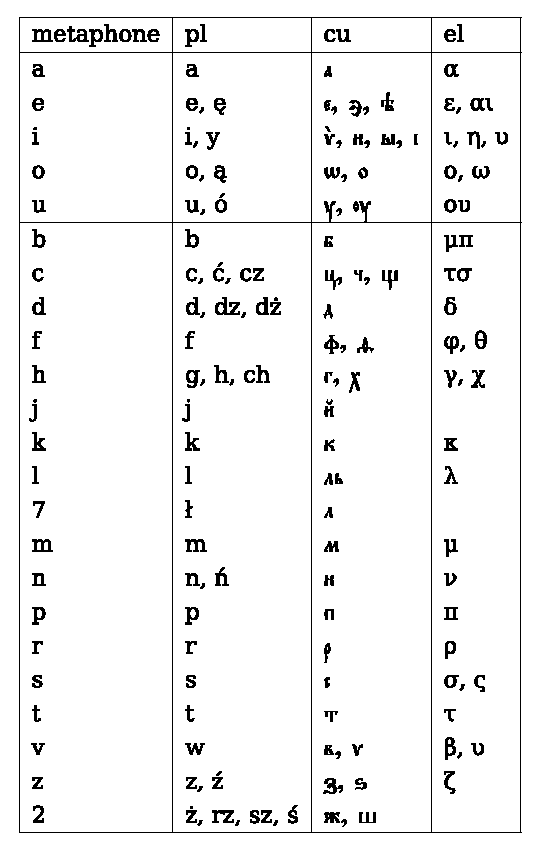
\includegraphics[width=2.5in]{metaphone.eps}
  \label{tab:metaphone}
\end{table}

\begin{table}
  \small
  \caption{Przykładowe klucze Metaphone i~przykłady słów im przyporządkowanych}
  \centering
  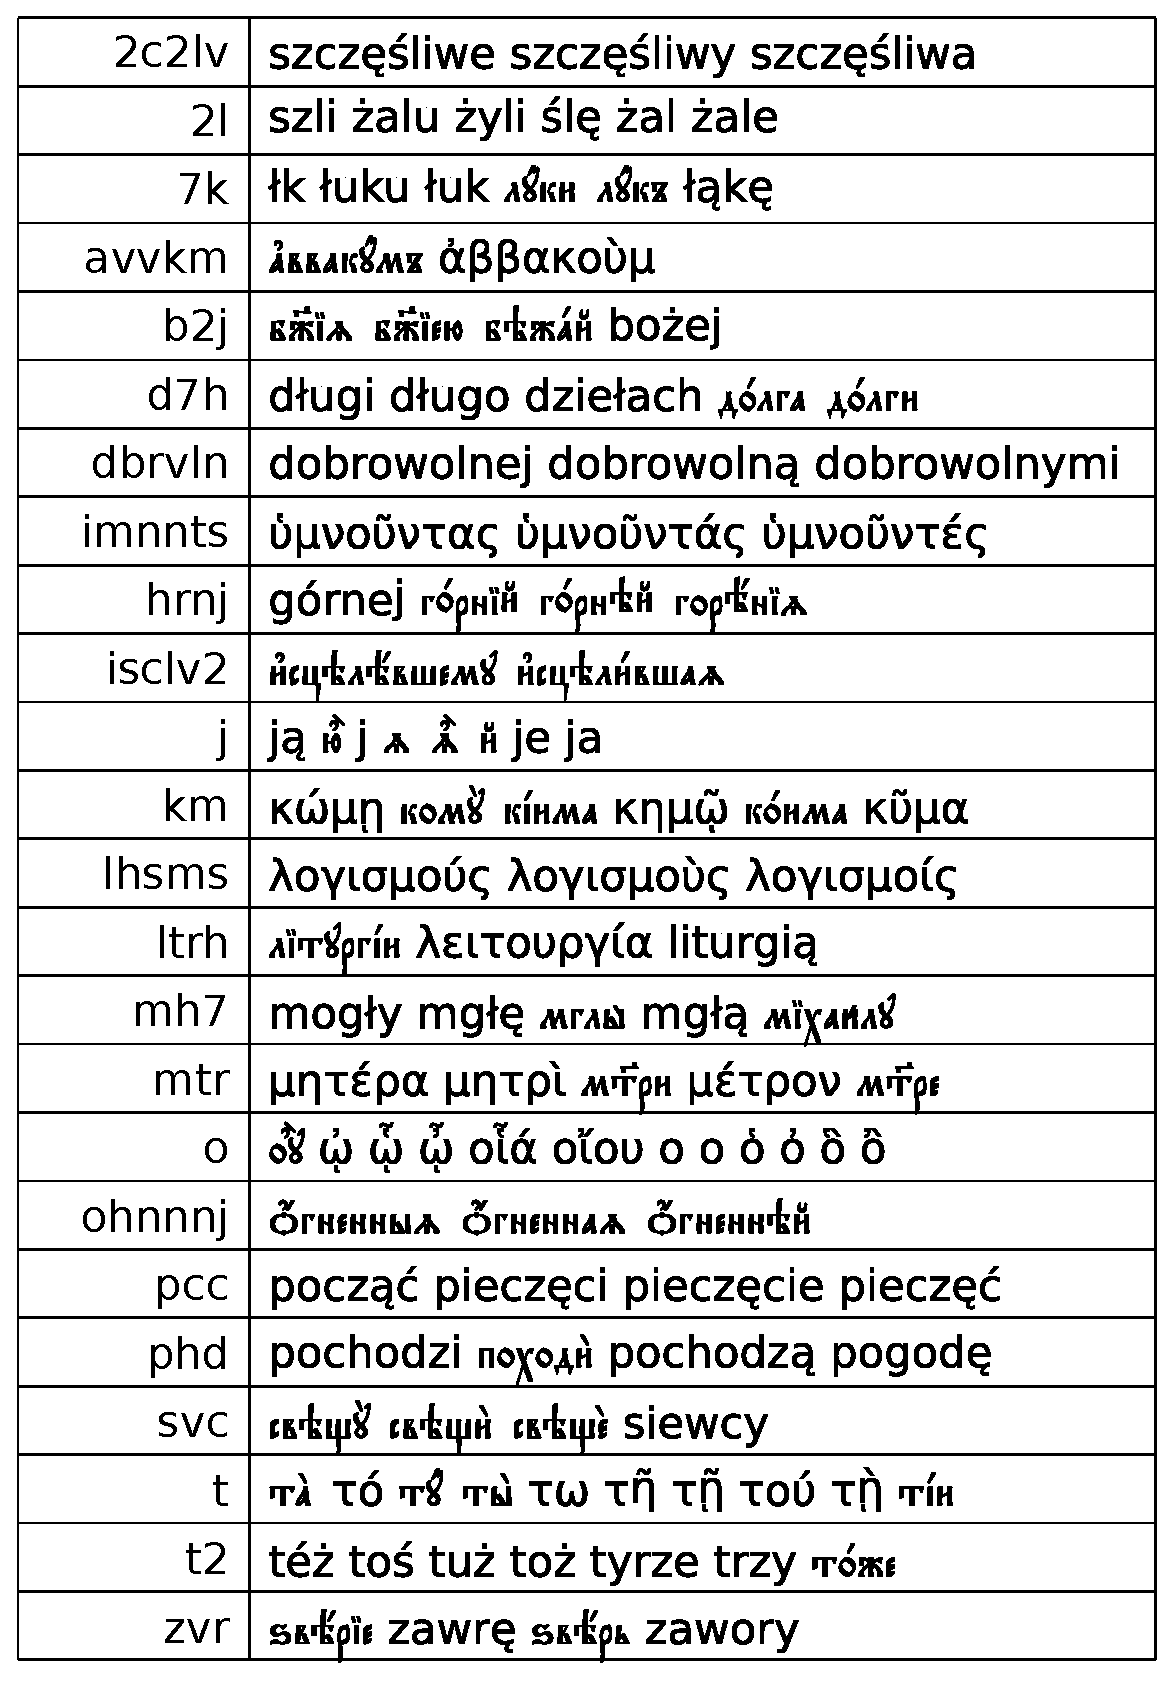
\includegraphics[width=2.5in]{metaphone2.eps}
  \label{tab:metaphone2}
\end{table}


\section{Przeszukiwarka}

Przeszukiwarka korpusu została zaimplementowana przy pomocy biblioteki
Whoosh \cite{whoosh}. Aby możliwe było szybkie przeszukiwanie,
najpierw tworzy się indeks bazujący na kluczach metaphone kolejnych
słów tekstu, a następnie, przy wyszukiwaniu, otrzymujemy jako wyjście
nazwę pliku i numer zdania, w którym zostało znalezione wyszukiwane
słowo. Jets to używane do wyświetlenia kontekstu w wynikach wyszukiwania.


\section{Interfejs wiersza poleceń}\label{r:cli}

Większość modułów pakietu {\tt toolkit} udostępnia swoją
funkcjonalność poprzez prosty interfejs wiersza poleceń. Większość
skryptów przy uruchomieniu bez argumentów wyświetla pomoc lub inne
pożyteczne informacje. Wymienię poniżej kilka istotniejszych z~nich:

\paragraph{{\tt fetcher}}
Fetcher pobiera odpowiedni tekst lub dopasowanie tekstów i~wypisuje go
(w odpowiednio sformatowanej postaci) na standardowe wyjście.

\paragraph{{\tt search}}
Skrypt przeszukuje bazę tekstów i~wyświetla wynik. Wywołanie go
z~opcją {\tt --create-index} powoduje utworzenie indeksu potrzebnego do
realizacji wyszukiwania. Wyszukiwarka opiera się na bibliotece Whoosh
\cite{whoosh}.

\paragraph{{\tt aligner}}
Dopasowuje do siebie 2 teksty. Na uwagę zasługują opcje {\tt --hand},
{\tt --prealign} i~{\tt --plot}. Opcja {\tt --hand} pozwala wymusić
dopasowanie pewnych par zdań, tak, żeby ,,nakierować'' program na
właściwą ścieżkę dopasowania. Opcja {\tt --prealign} działa podobnie,
lecz tutaj te pary zdań wyszukiwane są automatycznie. Wreszcie opcje
{\tt --plot} i~{\tt --plot-sim} pozwalają na wygenerowanie wykresu
podobnego do tego przedstawionego na rys. \ref{fig:matrix}.

\paragraph{{\tt Alignment}}
Skrypt Alignment.py zawiera klasę obsługującą dopasowania wielu
tekstów. Wywołany samodzielnie z~wiersza poleceń, wyświetla podany
plik dopasowania. Fragment przykładowego wyniku działania skryptu
można zobaczyć na rysunku \ref{f:alignment}.

\begin{figure}[h]
  \small
  \caption{Przykładowe dopasowanie tekstów wyświetlone w~konsoli.}
  \centering
    \includegraphics[width=5in]{console-alignment.png}
    \label{f:alignment}
\end{figure}

\paragraph{Pakiet {\tt translit}}
Wszystkie skrypty z~pakietu {\tt translit} można uruchomić z~wiersza
poleceń, aby dokonać odpowiedniej transliteracji na wybranym
tekście. Jako argument należy podać plik z~tekstem, lub {\tt -}, aby
korzystać ze standardowego wejścia. Dostępnie są następujące skrypty:

\begin{itemize}
\item {\tt expand\_cu.py} -- rozwijanie skrótów języka
  cerkiewno\-{}słowiańskiego i~konwersja liczb na cyfry arabskie,
\item {\tt cu2pl.py} -- transkrypcja fonetyczna języka
  cerkiewno\-{}słowiańskiego na polski,
\item {\tt render\_cu.py} -- konwersja tekstu
  cerkiewno\-{}słowiańskiego do formatu UCS (patrz dodatek
  \ref{encoding}),
\item {\tt simplify\_el.py} -- ujednolicanie greckich akcentów
  i~usuwanie innych znaków diakrytycznych,
\item {\tt el2pl.py} -- transkrypcja fonetyczna z~(,,uproszczonego'')
  greckiego na polski,
\item {\tt metaphone.py} -- zamiana tekstu na ciąg kluczy Metaphone.
\end{itemize}


\section{Interfejs internetowy}\label{r:www}

Do utworzenia interfejsu internetowego użyłem frameworka Django
\cite{django}. Zdecydowałem się na ten wybór, ponieważ cały kod mojego
projektu został napisany w~Pythonie, a Django jest najpopularniejszym
frameworkiem do tworzenia aplikacji internetowych w~Pythonie, i~miałem
z~nim styczność podczas zajęć na MIM UW.

Interfejs internetowy można uruchomić do przetestowania wpisując
polecenie {\tt ./www/manage.py runserver} w~terminalu w~głównym
katalogu projektu. Powoduje to uruchomienie serwera HTTP, który
odpowiada na zapytania pod adresem \url{http://127.0.0.1:8000/}.

Wygląd przykładowej strony można zobaczyć na rys. \ref{f:web2}.

\begin{figure}[h]
  \small
  \caption{Widok tekstu w~interfejsie internetowym}
  \includegraphics[width=\textwidth]{web2.png}
  \label{f:web2}
\end{figure}

\paragraph{Model}
Model danych i~operacje na nich obsługuje napisany przeze mnie pakiet
{\tt toolkit}. Nie potrzebowałem używać baz danych, które zwykle są
pomocne w~podobnych projektach.

\paragraph{Widoki}
Cały serwis internetowy obsługują 3 widoki.

\begin{itemize}
\item \textbf{Widok tekstu} -- Wyświetla tekst równoległy (widoczny na
  rys. \ref{f:web2}). Po lewej stronie znajdują się pola wyboru
  języków, których zmiana powoduje przeładowanie strony z~nowymi
  ustawieniami.
\item \textbf{Widok katalogu} -- Wyświetla spis treści książki lub spis
  książek.  To zadanie sprowadza się do wyświetlenia odpowiednio
  sformatowanej listy plików (rys. \ref{f:dir}).
\item \textbf{Widok wyników wyszukiwania} -- Wyświetla wyniki
  przeszukiwania korpusu (rys. \ref{f:search}).
\end{itemize}

\begin{figure}[h]
  \small \centering
  \caption{Widok katalogu}
  \includegraphics[width=3in]{webfolder.png}
  \label{f:dir}
\end{figure}

\begin{figure}[h]
  \small \centering
  \caption{Widok wyników wyszukiwania}
  \includegraphics[width=3in]{websearch.png}
  \label{f:search}
\end{figure}

\paragraph{Szablony}
Szablony są prostymi plikami HTML, korzystającymi z~zewnętrznych
arkuszy stylów CSS i~skryptów w~JavaScripcie. Aby umożliwić
przeglądanie tekstów cerkiewno\-{}słowiańskich osobom, które nie mają
zainstalowanej w~systemie odpowiedniej czcionki, użyłem deklaracji
{\tt @font-face} z~języka opisu formy prezentacji stron WWW
CSS. Deklaracja ta wprowadzona została dopiero w~wersji 3 standardu,
dlatego może nie działać w~starszych przeglądarkach. Jednak nowe
wersje wszystkich wiodących przeglądarek (Firefox 3.6+, Opera
10.0+, Chrome 2.0+, Safari 4.0+, Internet Explorer 9+) obsługują ją
poprawnie. Starsze wersje Internet Explorera wyświetlają odstępy pod
znakami diakrytycznymi, jednak zawsze można ten problem obejść,
wyświetlając tekst w~transkrypcji fonetycznej.

\paragraph{Skrypty}
Zmiana języków jest obsługiwana przez krótki skrypt w~języku
JavaScript. Preferencje użytkownika są zapisywane w~pliku cookie
i~odczytywane przy następnej wizycie. Podświetlanie odpowiadających
sobie fragmentów tekstu jest również obsługiwane przez skrypt
JavaScript.

\section{Zakończenie}

Skromnym zdaniem autora, w pracy została zrealizowana większość celów,
o których mowa we wprowadzeniu. Wiele detali wciąż wymaga
dopracowania, jednak najważniejsza funkcjonalność została
zaimplementowana i przetestowana. Jeśli stworzony serwis zostanie
opublikowany w internecie, z pewnością pomoże to w~jego dalszym
rozwoju.

%%%%%%%%%%%%%%%%%%%%%%%%%%%%%%%%%%%%%%%%%%%%%%%%%%%%%%%%%%%%%%%%%%%%%%

\appendix

\chapter{Spis zawartości płyty}

Na dołączonej płycie zostały zapisane następujące pliki i katalogi:

\begin{itemize}
\item {\tt /praca\_magisterska.pdf} -- niniejsza praca,
\item {\tt /corthus/} -- główny katalog projektu,
\item {\tt /corthus/toolkit/} -- główna funkcjonalność projektu,
\item {\tt /corthus/www/} -- interfejs internetowy,
\item {\tt /corthus/texts/} -- baza tekstów,
\item {\tt /corthus/data/} -- pamięć tłumaczeniowa,
\item {\tt /corthus/index/} -- indeks wyszukiwania,
\item {\tt /corthus/external/} -- zewnętrzne biblioteki i~narzędzia.
\end{itemize}

%%%%%%%%%%%%%%%%%%%%%%%%%%%%%%%%%%%%%%%%%%%%%%%%%%%%%%%%%%%%%%%%%%%%%%

\chapter{Formaty plików}\label{r:formaty}

\section{HIP i~UCS -- tekst cerkiewno\-{}słowiański}
\label{encoding}

W~czasach, kiedy więszość tekstów cerkiewno\-{}słowiańskich została
zdigitalizowanych, standard Unicode nie zawierał wszystkich znaków
potrzebych do zapisu tekstu w~języku cerkiewno\-{}słowiańskim.
W~odpowiedzi na to powstał standard HIP (opisany dokładnie w~internecie
na stronie \cite{hip}). Pliki HIP to pliki tekstowe kodowane w
Windows-1251, używające cyrylicy wraz z~niektórymi literami
łacińskimi, aby w~ten sposób wyrazić wszystkie litery alfabetu
cerkiewno\-{}słowiańskiego. Zapis poszczególnych liter alfabetu (różne
warianty zapisu) zostały przedstawione w~tabeli \ref{tab:hip}.

\begin{table}[ht!]
  \small
  \caption{Kodowanie znaków cerkiewno\-{}słowiańskich w~standardzie HIP}
  \centering
    \includegraphics[width=\textwidth]{HIP-tabelka.png}
    \label{tab:hip}
\end{table}

Brakujące znaki były stopniowo dodawane do Unicode w~wersjach 5.0.0
(2006), 5.1.0 (2008) i~5.2.0 (2009). Można więc obecnie zapisać tekst
cerkiewno\-{}słowiański w~Unicode -- głównym problemem jest jednak
dostępność czcionek: czcionki obsługujące tytła literowe (znaki {\tt
  2DE0-2DFF}) i~literę {\cyr ꙋ} ({\tt A64B}) są wielką rzadkością. Na
chwilę obecną udało mi się w~internecie znaleźć tylko jedną czcionkę
obsługującą w~pełni język cerkiewno\-{}słowiański, oznaczoną jako
,,wersja beta'' \cite{ponomar}. Używam wobec tego starszych czcionek,
dostosowanych do kodowania UCS. Kodowanie UCS jest oparte na
Windows-1251. Znaki cyrylicy są w~nim kodowane tak samo, jednak
wszystkie pozostałe pozycje strony kodowej są zajęte przez pozostałe
znaki języka cerkiewno\-{}słowiańskiego oraz ligatury tych znaków
z~tytłami lub znakami diakrytycznymi (tylko w~zestawieniach, gdzie takie
ligatury są potrzebne).

Dużą wadą takiego kodowania jest to, że jest ono niekompatybilne
z~ASCII, i~tak zakodowany tekst jest czytelny tylko jeśli zostanie
wyświetlony odpowiednią czcionką. Przykładowe czcionki dla tego
kodowania można pobrać ze strony \textit{Irmologion}
\cite{irmologion}.

\section{TXT -- pliki tekstowe}

Wszystkie pliki TXT w~projekcie są kodowane w~UTF-8. Zdecydowałem
jednak nie konwertować tekstów cerkiewno\-{}słowiańskich z~zapisu HIP na
znaki odpowiadające im wedug standardu Unicode, ze względu na problemy
z~wyświetlaniem tych znaków (patrz punk \ref{encoding}). Ta decyzja
pozwoliła mi na duże uproszczenie logiki programu, bo mogłem bardzo
łatwo przeglądać te pliki i~wprowadzać w~nich zmiany. Wadami tego
rozwiązania była konieczność rezygnacji z~formatowania i~nieco większy
rozmiar plików.

Połamałem akapity na linie nie dłuższe niż 70 znaków, rozdzielając
akapity od siebie pustymi liniami (analogicznie do TeXa), tak żeby można
było je wygodnie przeglądać w~dowolnym edytorze tekstu lub w~konsoli.

\section{Pliki dopasowań}

Dopasowania tekstów są zapisywane w~formacie CSV, z~tabulatorem
pełniącym rolę separatora pól. Jest to dokładnie taki format, jaki
zwraca Hunalign.

Nazwy plików dopasowań kończą się rozszerzeniem {\tt .hunalign}, {\tt
  .my} lub {\tt .golden}, w~zależności od swojego pochodzenia. Kolejne
rozszerzenia oznaczają odpowiednio pliki wygenerowane przez Hunaligna,
pliki utworzone przez aligner z~projektu i~pliki dopasowań utworzone
ręcznie.

\chapter{Licencja Apache 2.0}\label{r:licencja}

\small

{\centering
  Apache License\\
  Version 2.0, January 2004\\
  \url{http://www.apache.org/licenses/}\\
  \textbf{TERMS AND CONDITIONS FOR USE, REPRODUCTION, AND DISTRIBUTION}\\
}

\begin{enumerate}

\item \textbf{Definitions}.

  ``License'' shall mean the terms and conditions for use, reproduction,
  and distribution as defined by Sections 1 through 9 of this
  document.

  ``Licensor'' shall mean the copyright owner or entity authorized by
  the copyright owner that is granting the License.

  ``Legal Entity'' shall mean the union of the acting entity and all
  other entities that control, are controlled by, or are under common
  control with that entity. For the purposes of this definition,
  ``control'' means (i) the power, direct or indirect, to cause the
  direction or management of such entity, whether by contract or
  otherwise, or (ii) ownership of fifty percent (50\%) or more of the
  outstanding shares, or (iii) beneficial ownership of such entity.

  ``You'' (or ``Your'') shall mean an individual or Legal Entity
  exercising permissions granted by this License.

  ``Source'' form shall mean the preferred form for making
  modifications, including but not limited to software source code,
  documentation source, and configuration files.

  ``Object'' form shall mean any form resulting from mechanical
  transformation or translation of a Source form, including but not
  limited to compiled object code, generated documentation, and
  conversions to other media types.

  ``Work'' shall mean the work of authorship, whether in Source or
  Object form, made available under the License, as indicated by a
  copyright notice that is included in or attached to the work (an
  example is provided in the Appendix below).

  ``Derivative Works'' shall mean any work, whether in Source or Object
  form, that is based on (or derived from) the Work and for which the
  editorial revisions, annotations, elaborations, or other
  modifications represent, as a whole, an original work of
  authorship. For the purposes of this License, Derivative Works shall
  not include works that remain separable from, or merely link (or
  bind by name) to the interfaces of, the Work and Derivative Works
  thereof.

  ``Contribution'' shall mean any work of authorship, including the
  original version of the Work and any modifications or additions to
  that Work or Derivative Works thereof, that is intentionally
  submitted to Licensor for inclusion in the Work by the copyright
  owner or by an individual or Legal Entity authorized to submit on
  behalf of the copyright owner. For the purposes of this definition,
  ``submitted'' means any form of electronic, verbal, or written
  communication sent to the Licensor or its representatives, including
  but not limited to communication on electronic mailing lists, source
  code control systems, and issue tracking systems that are managed
  by, or on behalf of, the Licensor for the purpose of discussing and
  improving the Work, but excluding communication that is
  conspicuously marked or otherwise designated in writing by the
  copyright owner as ``Not a Contribution.''

  ``Contributor'' shall mean Licensor and any individual or Legal Entity
  on behalf of whom a Contribution has been received by Licensor and
  subsequently incorporated within the Work.

\item \textbf{Grant of Copyright License}. Subject to the terms and
  conditions of this License, each Contributor hereby grants to You a
  perpetual, worldwide, non-exclusive, no-charge, royalty-free,
  irrevocable copyright license to reproduce, prepare Derivative Works
  of, publicly display, publicly perform, sublicense, and distribute
  the Work and such Derivative Works in Source or Object form.

\item \textbf{Grant of Patent License}. Subject to the terms and
  conditions of this License, each Contributor hereby grants to You a
  perpetual, worldwide, non-exclusive, no-charge, royalty-free,
  irrevocable (except as stated in this section) patent license to
  make, have made, use, offer to sell, sell, import, and otherwise
  transfer the Work, where such license applies only to those patent
  claims licensable by such Contributor that are necessarily infringed
  by their Contribution(s) alone or by combination of their
  Contribution(s) with the Work to which such Contribution(s) was
  submitted. If You institute patent litigation against any entity
  (including a cross-claim or counterclaim in a lawsuit) alleging that
  the Work or a Contribution incorporated within the Work constitutes
  direct or contributory patent infringement, then any patent licenses
  granted to You under this License for that Work shall terminate as
  of the date such litigation is filed.

\item \textbf{Redistribution}. You may reproduce and distribute copies
  of the Work or Derivative Works thereof in any medium, with or
  without modifications, and in Source or Object form, provided that
  You meet the following conditions:

  \begin{enumerate}[label=(\alph*)]
  \item You must give any other recipients of the Work or
    Derivative Works a copy of this License; and

  \item You must cause any modified files to carry prominent notices
    stating that You changed the files; and

  \item You must retain, in the Source form of any Derivative Works
    that You distribute, all copyright, patent, trademark, and
    attribution notices from the Source form of the Work, excluding
    those notices that do not pertain to any part of the Derivative
    Works; and

  \item If the Work includes a ``NOTICE'' text file as part of its
    distribution, then any Derivative Works that You distribute must
    include a readable copy of the attribution notices contained
    within such NOTICE file, excluding those notices that do not
    pertain to any part of the Derivative Works, in at least one of
    the following places: within a NOTICE text file distributed as
    part of the Derivative Works; within the Source form or
    documentation, if provided along with the Derivative Works; or,
    within a display generated by the Derivative Works, if and
    wherever such third-party notices normally appear. The contents of
    the NOTICE file are for informational purposes only and do not
    modify the License. You may add Your own attribution notices
    within Derivative Works that You distribute, alongside or as an
    addendum to the NOTICE text from the Work, provided that such
    additional attribution notices cannot be construed as modifying
    the License.
  \end{enumerate}

  You may add Your own copyright statement to Your modifications and
  may provide additional or different license terms and conditions for
  use, reproduction, or distribution of Your modifications, or for any
  such Derivative Works as a whole, provided Your use, reproduction,
  and distribution of the Work otherwise complies with the conditions
  stated in this License.

\item \textbf{Submission of Contributions}. Unless You explicitly
  state otherwise, any Contribution intentionally submitted for
  inclusion in the Work by You to the Licensor shall be under the
  terms and conditions of this License, without any additional terms
  or conditions.  Notwithstanding the above, nothing herein shall
  supersede or modify the terms of any separate license agreement you
  may have executed with Licensor regarding such Contributions.

\item \textbf{Trademarks}. This License does not grant permission to
  use the trade names, trademarks, service marks, or product names of
  the Licensor, except as required for reasonable and customary use in
  describing the origin of the Work and reproducing the content of the
  NOTICE file.

\item \textbf{Disclaimer of Warranty}. Unless required by applicable
  law or agreed to in writing, Licensor provides the Work (and each
  Contributor provides its Contributions) on an ``AS IS'' BASIS, WITHOUT
  WARRANTIES OR CONDITIONS OF ANY KIND, either express or implied,
  including, without limitation, any warranties or conditions of
  TITLE, NON-INFRINGEMENT, MERCHANTABILITY, or FITNESS FOR A
  PARTICULAR PURPOSE. You are solely responsible for determining the
  appropriateness of using or redistributing the Work and assume any
  risks associated with Your exercise of permissions under this
  License.

\item \textbf{Limitation of Liability}. In no event and under no legal
  theory, whether in tort (including negligence), contract, or
  otherwise, unless required by applicable law (such as deliberate and
  grossly negligent acts) or agreed to in writing, shall any
  Contributor be liable to You for damages, including any direct,
  indirect, special, incidental, or consequential damages of any
  character arising as a result of this License or out of the use or
  inability to use the Work (including but not limited to damages for
  loss of goodwill, work stoppage, computer failure or malfunction, or
  any and all other commercial damages or losses), even if such
  Contributor has been advised of the possibility of such damages.

\item \textbf{Accepting Warranty or Additional Liability}. While
  redistributing the Work or Derivative Works thereof, You may choose
  to offer, and charge a fee for, acceptance of support, warranty,
  indemnity, or other liability obligations and/or rights consistent
  with this License. However, in accepting such obligations, You may
  act only on Your own behalf and on Your sole responsibility, not on
  behalf of any other Contributor, and only if You agree to indemnify,
  defend, and hold each Contributor harmless for any liability
  incurred by, or claims asserted against, such Contributor by reason
  of your accepting any such warranty or additional liability.

\end{enumerate}

%%%%%%%%%%%%%%%%%%%%%%%%%%%%%%%%%%%%%%%%%%%%%%%%%%%%%%%%%%%%%%%%%%%%%%

\begin{thebibliography}{99}
\addcontentsline{toc}{chapter}{Bibliografia}

\bibitem{church+gale} Kenneth W. Church, William A. Gale, \textit{A
  Program for Aligning Sentences in Bilingual Corpora}, Association of
  Computational Linguistics, 1993

\bibitem{orthlib} Teksty cerkiewno\-{}słowiańskie:\\
  {\tt http://orthlib.ru/worship/}

\bibitem{analogion} Teksty starogreckie:\\
  {\tt http://analogion.gr/glt/}

\bibitem{liturgia} Teksty polskie:\\
  {\tt http://www.liturgia.cerkiew.pl/page.php?id=14}

\bibitem{hip} Opis standardu HIP (w jęz. rosyjskim):\\
  {\tt http://orthlib.ru/hip/hip-9.html}

\bibitem{ponomar} Projekt Ponomar \\
  {\tt http://www.ponomar.net/cu\_support.html}

\bibitem{irmologion} Czcionki z~ligaturami potrzebne do wyświetlania
  tekstów w~jęz. cerkiewno\-{}słowiańskim:\\
  {\tt http://www.irmologion.ru/fonts.html}

\bibitem{unicode}
  The Unicode Consortium. \textit{The Unicode Standard}.\\
  {\tt http://www.unicode.org/charts/PDF/U0400.pdf} (Cyrillic)\\
  {\tt http://www.unicode.org/charts/PDF/U2DE0.pdf} (Cyrillic Extended-A)\\
  {\tt http://www.unicode.org/charts/PDF/UA640.pdf} (Cyrillic Extended-B)

\bibitem{soundex} Algorytm Soundex:\\
  {\tt http://en.wikipedia.org/wiki/Soundex}

\bibitem{metaphone} Algorytm Metaphone:\\
  {\tt http://en.wikipedia.org/wiki/Metaphone},\\
  Hanging on the Metaphone, Lawrence Philips. Computer Language,
  Vol. 7, No. 12 (December), 1990.

\bibitem{giza} GIZA++\\
  {\tt http://code.google.com/p/giza-pp/}\\
  Franz Josef Och, Hermann Ney. \textit{"A Systematic Comparison of
  Various Statistical Alignment Models"},\\ \textit{Computational
  Linguistics}, volume 29, number 1, pp. 19-51 March 2003.

\bibitem{hunalign} Hunalign\\
  {\tt http://mokk.bme.hu/resources/hunalign/}\\
  D. Varga, L. Németh, P. Halácsy, A. Kornai, V. Trón, V. Nagy (2005).
  \textit{Parallel corpora for medium density languages},
  In Proceedings of the RANLP 2005, pages 590-596.

\bibitem{poliqarp} Poliqarp\\
  {\tt http://poliqarp.sourceforge.net/about.html}\\
  Adam Przepiórkowski. (2004). \textit{Korpus IPI PAN. Wersja
  wstępna}. IPI PAN, Warszawa.

\bibitem{strach} Stanisław Strach, \textit{Krótka gramatyka języka
  cerkiewno\-{}słowiańskiego}. Prawosławna Diecezja Białostocko-Gdańska,
  1994.

\bibitem{znosko} Aleksy Znosko, \textit{Słownik
  cerkiewno\-{}słowiańsko-polski}, Prawosławna Diecezja
  Białostocko-Gdańska, 1996.

\bibitem{django} Django core team (2011). \textit{Django: A Web
  framework for the Python programming language}. Django Software
  Foundation, Lawrence, Kansas, U.S.A. \\{\tt
    http://www.djangoproject.com}

\bibitem{whoosh} Whoosh Python Search Library\\
  {\tt https://bitbucket.org/mchaput/whoosh/wiki/Home}

\end{thebibliography}

\end{document}

